\chapter{Одноканальная система в форме вход-выход}
\label{ch:chap1}

\definecolor{codegreen}{rgb}{0,0.6,0}
\definecolor{codegray}{rgb}{0.5,0.5,0.5}
\definecolor{codepurple}{rgb}{0.58,0,0.82}
\definecolor{backcolour}{rgb}{0.95,0.95,0.92}

\lstdefinestyle{mystyle}{
    backgroundcolor=\color{backcolour},   
    commentstyle=\color{codegreen},
    keywordstyle=\color{magenta},
    numberstyle=\tiny\color{codegray},
    stringstyle=\color{codepurple},
    basicstyle=\ttfamily\footnotesize,
    breakatwhitespace=false,         
    breaklines=true,                 
    captionpos=b,                    
    keepspaces=true,                 
    numbers=left,                    
    numbersep=5pt,                  
    showspaces=false,                
    showstringspaces=false,
    showtabs=false,                  
    tabsize=2
}

\lstset{style=mystyle}


В случае моего второго варианта получим следующее ДУ:
$$
\begin{aligned}
    \dddot{y} + 6\ddot{y} + 11\dot{y} + 6y = 6\ddot{u} + 4\dot{u} + 16u
\end{aligned}
$$

Для того, чтобы составить структурную схему, выполним несколько преобразований с ДУ - заменим дифференцирования на применение соответсвующих операторов, а после преобразуем в более удобный вид:

$$
\begin{aligned}
    p^3[y] + 6p^2[y] + 11p[y] + 6y = 6p^2[u] + 4p[u] + 16u \\
	y = \frac{1}{p^3} \bigg[ -6p^2[y] - 11p[y] -6y + 6p^2[u] + 4p[u] + 16u \bigg] \\
	y = -6\frac{1}{p}[y] - 11\frac{1}{p^2}[y] -6\frac{1}{p^3}[y] + 6\frac{1}{p}[u] + 4\frac{1}{p^2}[u] + 16\frac{1}{p^3}[u] \\
	y = \frac{1}{p}[-6y + 6u] + \frac{1}{p^2}[-11y + 4u] \frac{1}{p^3}[-6y + 16u]
\end{aligned}
$$
Так как блок "дифференцирования" в матлабе - довольно опасная штука, то воспользуемся классическим приёмом составления схем: от обратного, постепенно снижая степень дифференцирования у "игрека" посредством интегрирования. Снизу мы построили передаточную функцию от ДУ, чтобы проверить результат симуляции:

\newpage
В итоге, структурная схема системы, построенная в \textit{Simulink}:

\begin{figure}[ht]
    \centering
    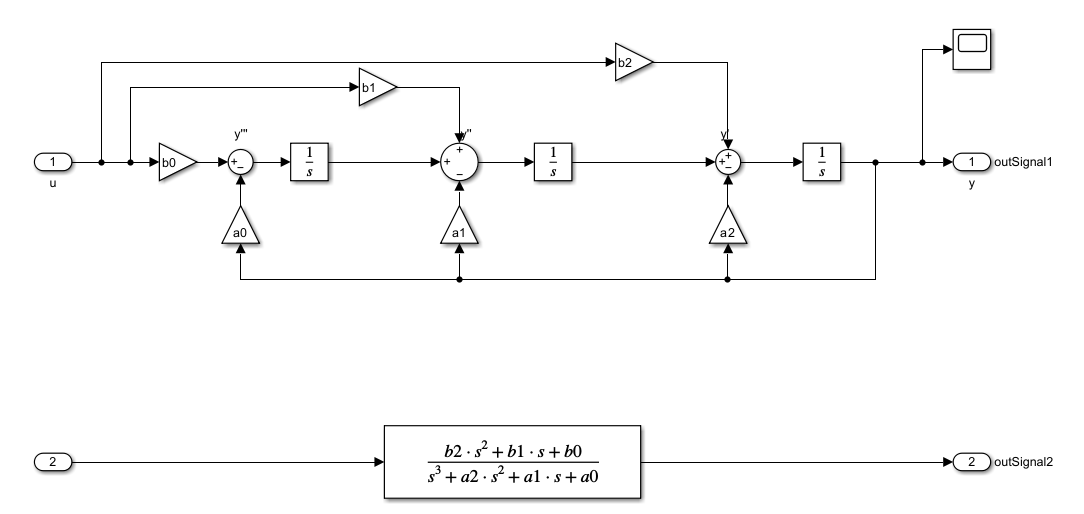
\includegraphics[width=1\textwidth]{scheme_task1.png}
	\caption{Схема системы}
\end{figure}

Подадим на такую схему сигнал $u(t)=1$ при нулевых начальных условиях: $\ddot{y}(0)=\dot{y}(0)=y(0)=0$. Графики сигналов, полученные на основе схемы:
\begin{figure}[h]
	\begin{subfigure}{0.5\textwidth}
		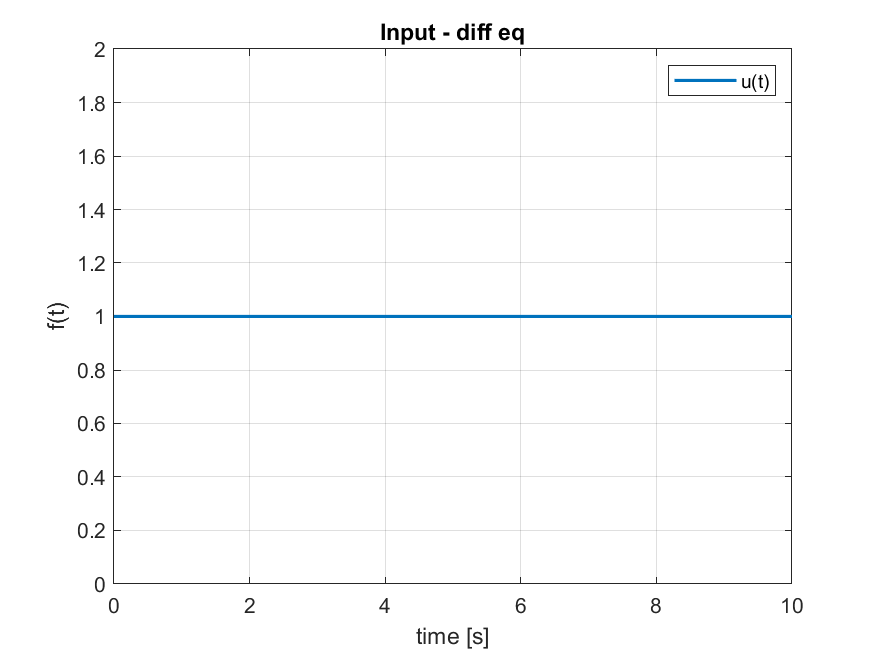
\includegraphics[width=0.9\linewidth, height=6cm]{input_task1_diff_eq.png} 
	\end{subfigure}
	\begin{subfigure}{0.5\textwidth}
		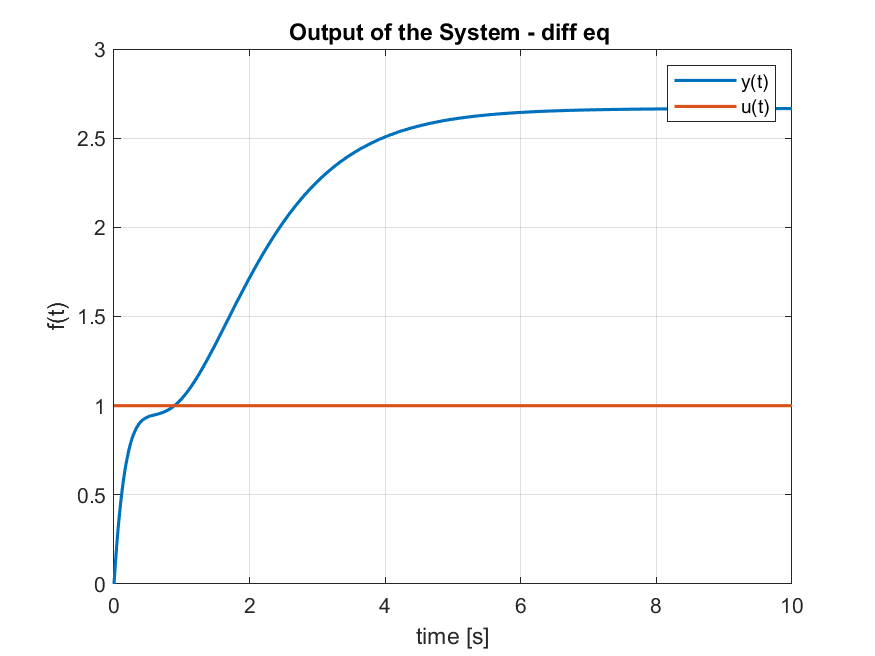
\includegraphics[width=0.9\linewidth, height=6cm]{output_task1_diff_eq.png}
	\end{subfigure}
	\caption{Симуляция - дифференциальное уравнение}
\end{figure}

\endinput